%%%%%%%%%%%%%%%%%%%%%%%%%%%%%%%%%%%%%%%%%
% Beamer Presentation
% LaTeX Template
% Version 1.0 (10/11/12)
%
% This template has been downloaded from:
% http://www.LaTeXTemplates.com
%
% License:
% CC BY-NC-SA 3.0 (http://creativecommons.org/licenses/by-nc-sa/3.0/)
%
%%%%%%%%%%%%%%%%%%%%%%%%%%%%%%%%%%%%%%%%%

%----------------------------------------------------------------------------------------
%	PACKAGES AND THEMES
%----------------------------------------------------------------------------------------

\documentclass{beamer}
\usepackage{xcolor}
\usepackage{lmodern}
\usepackage[ruled,vlined]{algorithm2e}
\usepackage{subcaption}
\usepackage{appendixnumberbeamer}

\mode<presentation> {

% The Beamer class comes with a number of default slide themes
% which change the colors and layouts of slides. Below this is a list
% of all the themes, uncomment each in turn to see what they look like.

% \usetheme{default}
% \usetheme{AnnArbor}
% \usetheme{Antibes}
% \usetheme{Bergen}
% \usetheme{Berkeley}
% \usetheme{Berlin}
%\usetheme{Boadilla}
\usetheme{CambridgeUS}
%\usetheme{Copenhagen}
%\usetheme{Darmstadt}
%\usetheme{Dresden}
%\usetheme{Frankfurt}
%\usetheme{Goettingen}
%\usetheme{Hannover}
%\usetheme{Ilmenau}
%\usetheme{JuanLesPins}
%\usetheme{Luebeck}
%\usetheme{Madrid}
%\usetheme{Malmoe}
%\usetheme{Marburg}
%\usetheme{Montpellier}
%\usetheme{PaloAlto}
% \usetheme{Pittsburgh}
%\usetheme{Rochester}
%\usetheme{Singapore}
%\usetheme{Szeged}
%\usetheme{Warsaw}

% As well as themes, the Beamer class has a number of color themes
% for any slide theme. Uncomment each of these in turn to see how it
% changes the colors of your current slide theme.

% \usecolortheme{albatross}
% \usecolortheme{beaver}
% \usecolortheme{beetle}
% \usecolortheme{crane}
\usecolortheme{dolphin} % OK
% \usecolortheme{dove}
% \usecolortheme{fly}
% \usecolortheme{lily} % OK, red and grey
% \usecolortheme{orchid} % OK, red and grey with blocks blue
% \usecolortheme{rose} % OK, red and grey with light blue blocks
% \usecolortheme{seagull}
% \usecolortheme{seahorse}
% \usecolortheme{whale}
% \usecolortheme{wolverine}

% \setbeamertemplate{footline} % To remove the footer line in all slides uncomment this line
%\setbeamertemplate{footline}[page number] % To replace the footer line in all slides with a simple slide count uncomment this line

\setbeamertemplate{navigation symbols}{} % To remove the navigation symbols from the bottom of all slides uncomment this line
\setbeamercovered{transparent}
}

\usepackage{graphicx} % Allows including images
\usepackage{booktabs} % Allows the use of \toprule, \midrule and \bottomrule in tables

%----------------------------------------------------------------------------------------
%	TITLE PAGE
%----------------------------------------------------------------------------------------

\title[Scholarly citations in Wikipedia]{An analysis of scholarly citations in Wikipedia} % The short title appears at the bottom of every slide, the full title is only on the title page

\author{Alessio Bogon} % Your name
\institute[University of Trento] % Your institution as it will appear on the bottom of every slide, may be shorthand to save space
{University of Trento \\ % Your institution for the title page
Department of Information Engineering and Computer Science \\
\medskip
Master Degree in Computer Science
}
\date{March 24, 2016} % Date, can be changed to a custom date


\begin{document}

\begin{frame}
\titlepage % Print the title page as the first slide
\end{frame}

\begin{frame}
\frametitle{Overview} % Table of contents slide, comment this block out to remove it
\tableofcontents % Throughout your presentation, if you choose to use \section{} and \subsection{} commands, these will automatically be printed on this slide as an overview of your presentation
\end{frame}

%----------------------------------------------------------------------------------------
%	PRESENTATION SLIDES
%----------------------------------------------------------------------------------------

%-----------------------------------------------------------------------------------------------------------------------------
\section{Introduction} % Sections can be created in order to organize your presentation into discrete blocks, all sections and subsections are automatically printed in the table of contents as an overview of the talk
\begin{frame}[c]
\Huge{\centerline{Introduction}}
\end{frame}

\subsection{Wikipedia}
\begin{frame}[c]{Wikipedia}
    \begin{columns}
        \column{.5\textwidth}
        \begin{itemize}
            \item Most used encyclopedia
            \item Started in 2001
            \item Studied by many
            \begin{itemize}
                \item Quality of citations~\cite{Nielsen2007}
                \item Illness prediction~\cite{McIver2014}
                \item Stock market moves strategy~\cite{Moat2013}
            \end{itemize}
        \end{itemize}
        \column{.4\textwidth}
        \begin{figure}
        \centering
        \includegraphics[width=\textwidth]{assets/wikipedian_protester}
        \caption{\centering Wikipedian protester (\url{xkcd.com/285})}
        \end{figure}
    \end{columns}
\end{frame}

%-----------------------------------------------------------------------------------------------------------------------------
\subsection{Open questions}

\begin{frame}
\frametitle{Open questions}
\begin{itemize}
    \item Quality of papers in Wikipedia, in term of:
    \begin{itemize}
        \item Incoming citations
        \item Journals rank
        \item Lifetime of citations
    \end{itemize}
    \item Prediction systems
    \begin{itemize}
        \item If a paper appears in Wikipedia, will it become more popular in the scientific community?
        \item In another way, do researcher use Wikipedia as their primary data source?
        \item Predict whether a publication is going to stay on a page
    \end{itemize}
\end{itemize}
\end{frame}

\subsection{Available datasets}
\begin{frame}{Available datasets}
\begin{itemize}
    \item Microsoft Academic Graph: a dataset containing data about papers, authors, references, journals, conferences, etc.
    \item Wikipedia dumps: text of all page revisions since the beginning
    \item Wikimedia hourly page view statistics
\end{itemize}
\end{frame}

\begin{frame}{Microsoft Academic Graph}
    \begin{itemize}
        \item Dataset powering the Microsoft Academic Search engine
        \item Size: 96 GB
        \item Contains over 120M papers (1800 -- 2016)
        \item Information about authors, references, journals, conferences, keywords, etc.
        \item Problems
        \begin{itemize}
            \item Only \emph{computer science} conferences
            \item Some of papers' publication dates are incomplete
            \item Not all the papers have a DOI (32\% of them)
        \end{itemize}
    \end{itemize}
\end{frame}

\subsection{The missing pieces}
\begin{frame}
\frametitle{The missing pieces}
\begin{itemize}
    \item History of papers appearing in Wikipedia (where and when)
    \item Usable/searchable page views dataset
\end{itemize}
\end{frame}

\section{Data manipulation}

\begin{frame}[c]
\Huge{\centerline{Data manipulation}}
\end{frame}

\subsection{Extracting citations from Wikipedia}
\begin{frame}{Extracting citations from Wikipedia}
    \begin{block}{Problems}
        \begin{itemize}
            \item Citations can be structured: \emph{wikimarkup} templates
            \begin{itemize}
                \item Many different variants
                \item Anybody can use custom macros
                \item Different templates for each language
            \end{itemize}
            \item or unstructured: plain text
            \begin{itemize}
                \item Recognize substrings that appear to be citations
            \end{itemize}
            \item Entity disambiguation
            \item Dataset size: 13,3 TB as of September 1st, 2015
        \end{itemize}
    \end{block}
    \begin{block}{Solution}
        \begin{itemize}
            \item Focus on publication identifiers (\emph{DOI}, \emph{PMID}, \emph{arXiv}, \emph{ISBN})
            \item The \textbf{wikidump} framework
        \end{itemize}
    \end{block}
\end{frame}

\begin{frame}
    \frametitle{Wikidump}
    \begin{columns}[t]
        \column{.6\textwidth}
        \begin{itemize}
            \item Facility framework to extract features from Wikipedia dumps
            \item Based on libraries by Aaron Halfaker
            \item Low memory consumption
            \item Highly parallelizable
            \item Written in Python
            \item[]
            \item Processed 445M page revisions (13,3~TB) in 21 hours
        \end{itemize}
        \column{.4\textwidth}
        \begin{table}
        \begin{tabular}{l r}
        \toprule
        \textbf{Type} & \textbf{Count} \\
        \midrule
        ISBN & 1\,153\,330 \\
        DOI & 651\,199 \\
        PMID & 372\,939 \\
        PMC & 79\,841 \\
        arXiv & 18\,832 \\
        \bottomrule
        \end{tabular}
        \caption{Number of identifiers extracted}
        \end{table}
    \end{columns}
\end{frame}

\subsection{Wikimedia page views}
\begin{frame}{Wikimedia page views}
    \begin{block}{Problems}
        \begin{itemize}
            \item Dataset size: 23 TB (4,7 TB for the 2014)
            \item Aggregated and ordered by hour (8670 files per year)
            \item They need to be cleaned
            \item They need to be \textbf{reordered}
            \item Unfeasible on a single machine
        \end{itemize}
    \end{block}
    \begin{block}{Solution}
        \begin{itemize}
            \item Exploit the UniTN Cisca Cluster
        \end{itemize}
    \end{block}
\end{frame}

\begin{frame}{The Spark job}
    \begin{itemize}
        \item UniTN Cisca Cluster
        \begin{itemize}
            \item 125 workstations
            \item 500 CPU cores in total
            \item Available only at night and in the weekend
        \end{itemize}
        \item The job
        \begin{itemize}
            \item Normalize the content
            \item Sample the first file
            \item Repartition the keyspace
            \item Sort each partition locally
        \end{itemize}
        \item[]
        \item Took one night for the 2014 dataset
        \item Took many nights to get it to work
    \end{itemize}
\end{frame}

\begin{frame}[c]{The Spark job --- Workflow}
    \begin{figure}
    \centering
    \includegraphics[width=0.9\textwidth]{assets/spark-pagecounts}
    \caption{Workflow showing the processing of Wikimedia page views}
    \end{figure}
\end{frame}


\section{Results}

\begin{frame}[c]
\Huge{\centerline{Results}}
\end{frame}

\begin{frame}{Quality of papers in Wikipedia}
\begin{itemize}
    \item Age of papers when inserted
    \item Incoming citations distribution
    \item Journals rank
    \item Lifetime of citations
\end{itemize}
\end{frame}

\subsection{Age of papers when inserted}
\begin{frame}{Age of papers when inserted}
    \begin{itemize}
        \item How old is a paper when it is insterted in Wikipedia for the first time?
        \item Interesting behavior of papers having few days
    \end{itemize}
\end{frame}

\subsection{Age of papers when inserted}
\begin{frame}{Age of papers when inserted}
    \begin{figure}
    \centering
    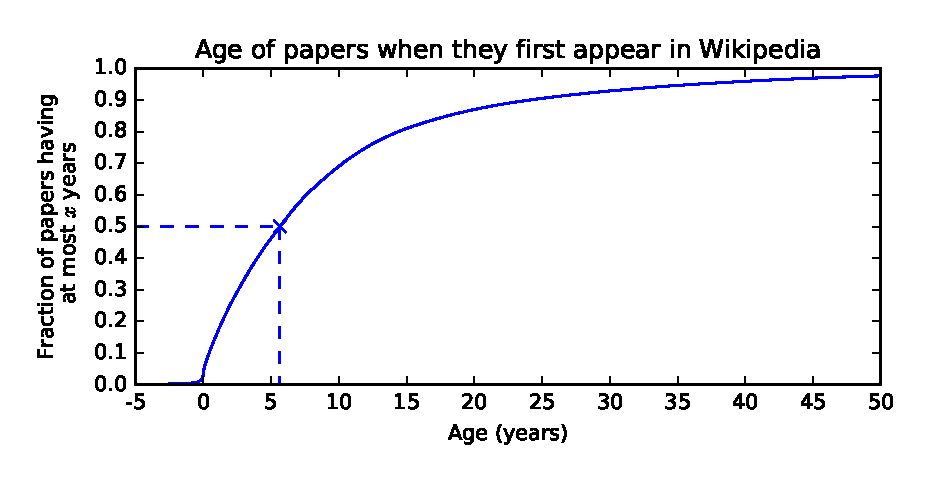
\includegraphics[width=0.9\textwidth]{assets/age_of_papers_at_first_appearance_cdf_slides}
    \end{figure}
\end{frame}

\begin{frame}{Age of papers when inserted --- Detail}
    \begin{figure}
    \centering
    \includegraphics[width=0.9\textwidth]{assets/age_of_papers_at_first_appearance_pdf_near0_slides}
    \end{figure}
    \centering
    1.3\% of papers are inserted within 7 days after the publication
\end{frame}


\subsection{Incoming citations distribution}
\begin{frame}{Incoming citations distribution}
    \begin{columns}
        \column{0.3\textwidth}
        \begin{itemize}
            \item Arguably follows a power law~\cite{Redner1998}: $N(x) \sim x^{-\alpha}$
            \item How well papers in Wikipedia perform?
        \end{itemize}
        \column{0.7\textwidth}
        \begin{figure}
        \centering
        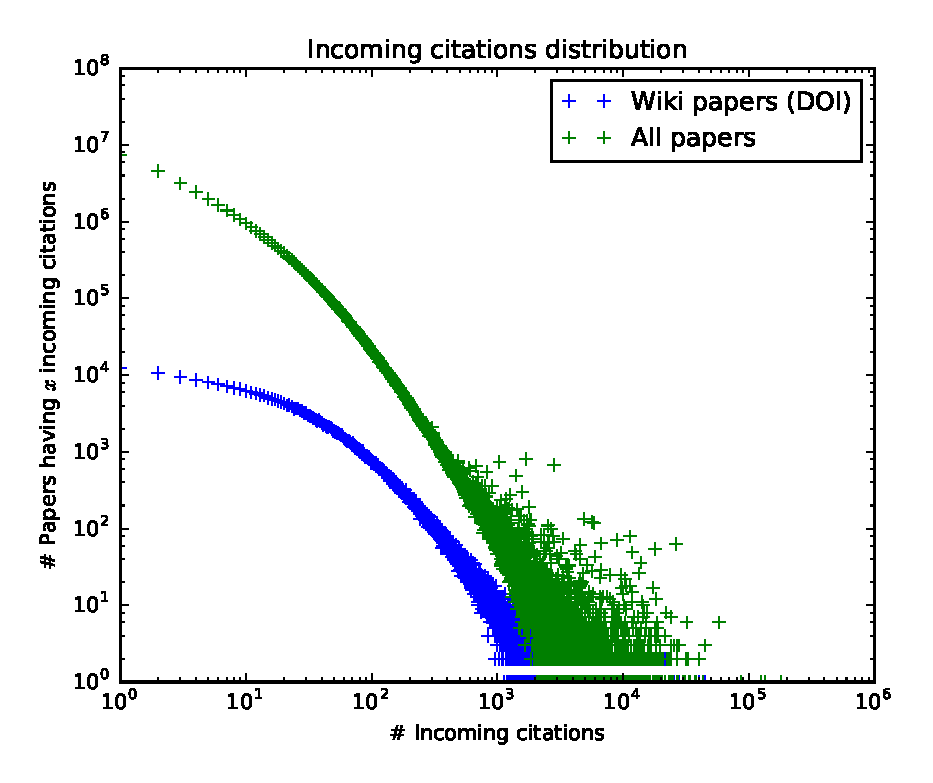
\includegraphics[width=1\textwidth]{assets/incoming_citations_distribution_pdf_slides}
        \end{figure}
    \end{columns}

\end{frame}

\begin{frame}{Incoming citations distribution}
    \begin{columns}
        \column{0.4\textwidth}
        \begin{itemize}
            \item Papers in Wikipedia behave like \emph{Genome Research} and \emph{PNAS}
            \item They outclass \emph{Nature} and \emph{Science}
            \item 75\% of papers in Wikipedia have more than 10 incoming citations
        \end{itemize}
        \column{0.6\textwidth}
        \begin{figure}
        \centering
        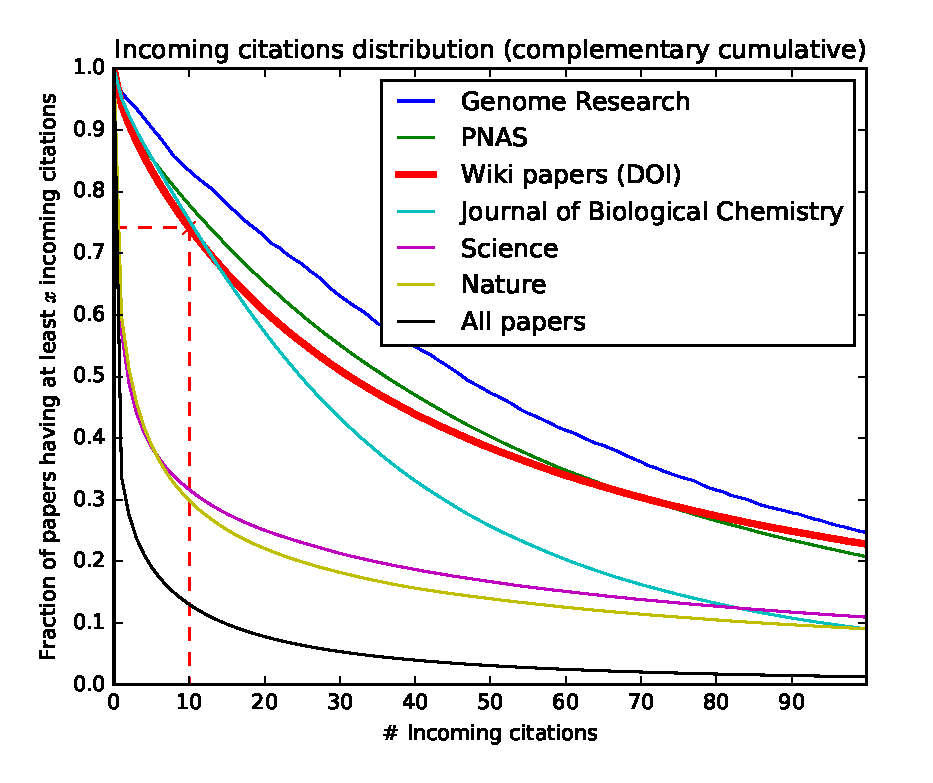
\includegraphics[width=1\textwidth]{assets/incoming_citations_distribution_ccdf_slides}
        \caption{Papers cited in Wikipedia vs papers in top journals}
        \end{figure}
    \end{columns}
\end{frame}

\subsection{Journals rank}
\begin{frame}{Journals rank}
    \begin{itemize}
        \item First proposed by Nielsen in 2007~\cite{Nielsen2007}
        \item Most cited journals in Wikipedia are also the most important ones
        \item[]
        \item Journals rank by impact factor versus:
        \begin{itemize}
            \item citations in Wikipedia
            \item visualizations in Wikipedia (in 2014)
        \end{itemize}
        \item Measured in term of Kendall rank correlation coefficient ($-1 \le \tau \le 1$)
    \end{itemize}
\end{frame}

\begin{frame}{Journals impact factor vs Wikipedia citations}
    \begin{figure}
    \centering
    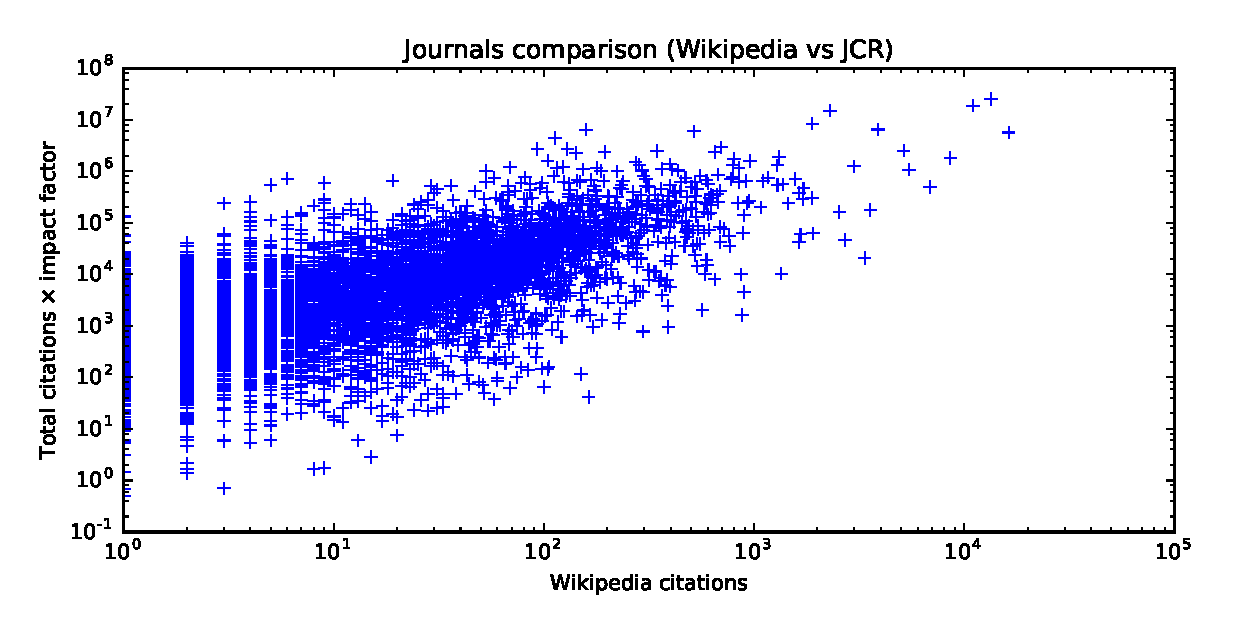
\includegraphics[width=0.9\textwidth]{assets/journals_compare_appearances}
    \end{figure}
    \centering
    Kendall rank correlation coefficient: $0.464$
\end{frame}

\begin{frame}{Journals impact factor vs Wikipedia impressions}
    \begin{figure}
    \centering
    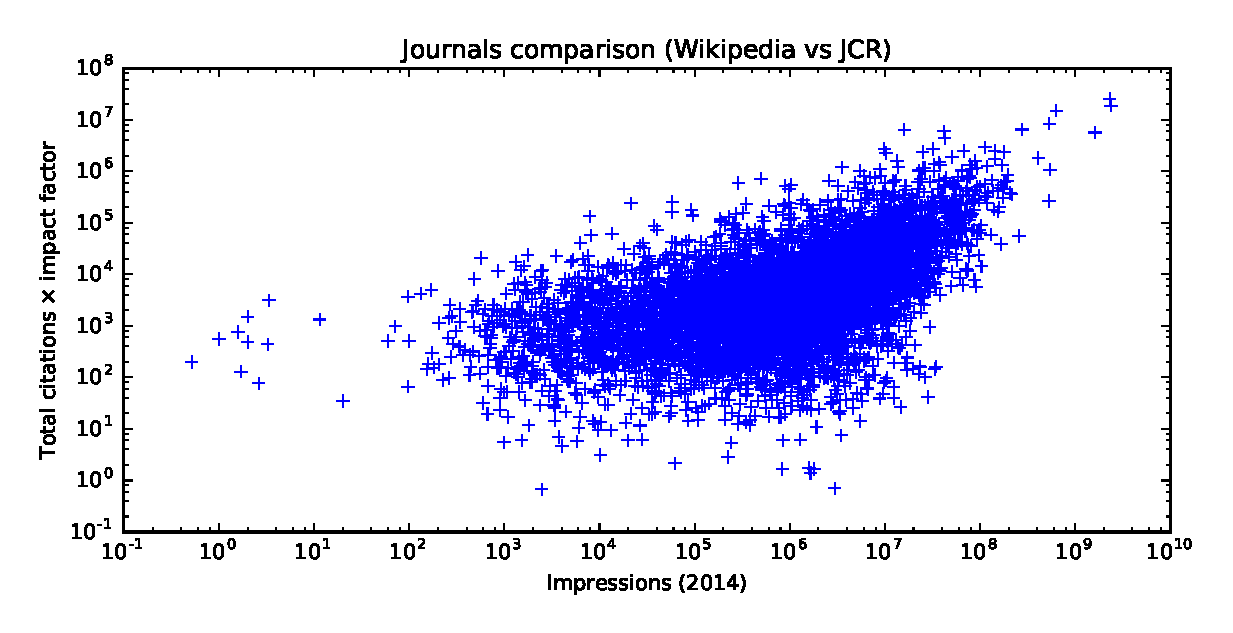
\includegraphics[width=0.9\textwidth]{assets/journals_compare_impressions2014}
    \end{figure}
    \centering
    Kendall rank correlation coefficient: $0.401$
\end{frame}

\begin{frame}{Maybe: Journals citations vs impressions in Wikipedia}
    \begin{figure}
    \centering
    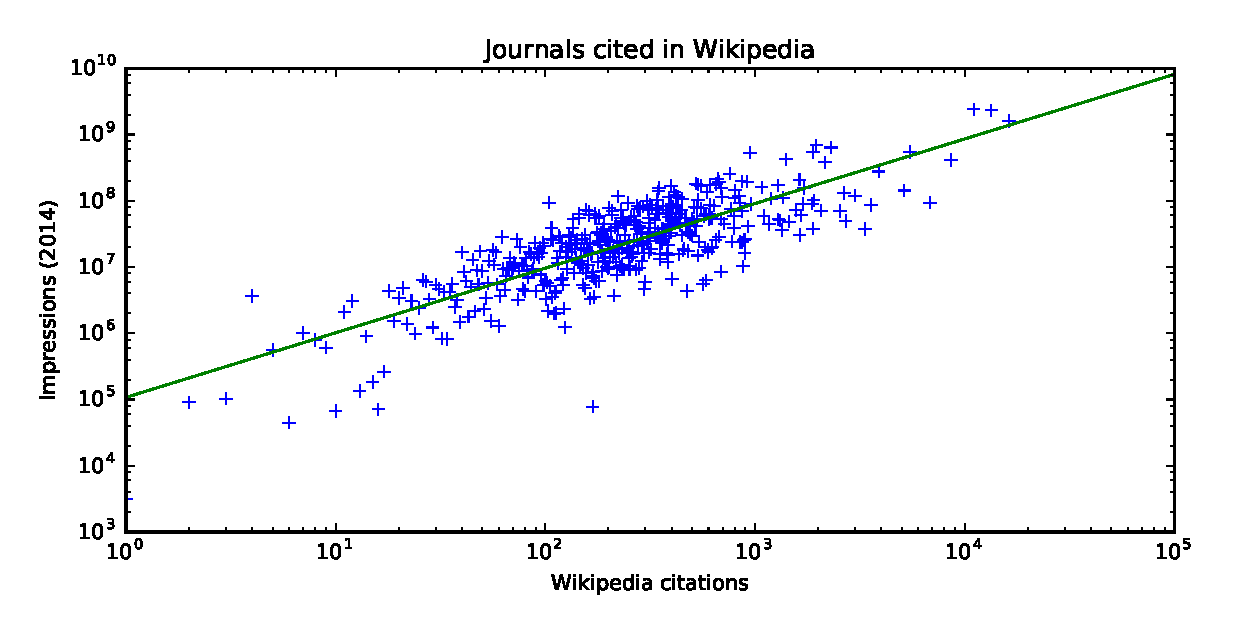
\includegraphics[width=0.9\textwidth]{assets/journals_appearances_impressions_loglog_slides}
    \end{figure}
    \centering
    Linear regression model: $\hat{y}_i = 10^{5.03} \times x^{0.98}$ ($r^2=0.65$)
\end{frame}

\subsection{Lifetime of irrelevant identifiers}
\begin{frame}{Lifetime of irrelevant identifiers}
    \begin{itemize}
        \item How long does it take for a Wikipedia contributor to discover and remove an ``irrelevant'' paper from an article?
        \item An identifier is ``irrelevant'' for an article if it appeared on that page and was then removed.
    \end{itemize}
\end{frame}

\begin{frame}
    \begin{columns}[c]
        \column{0.5\textwidth}
        \begin{itemize}
            \item Fraction of identifiers removed in time % (970\,273 in total)
            \item[]
            \item 60\% of irrelevant DOI removed within one year
            \item 35\% within one month
            \item 20\% within one day
        \end{itemize}
        \column{0.5\textwidth}
        \begin{figure}
        \centering
        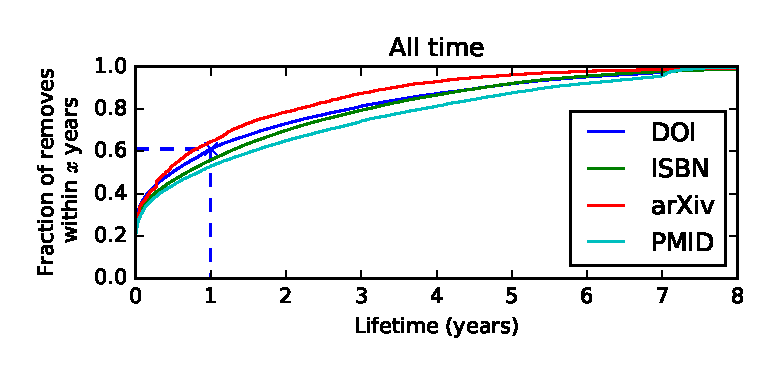
\includegraphics[width=1\textwidth]{assets/irrelevant_identifiers_persistence_cdf_max_slides}

        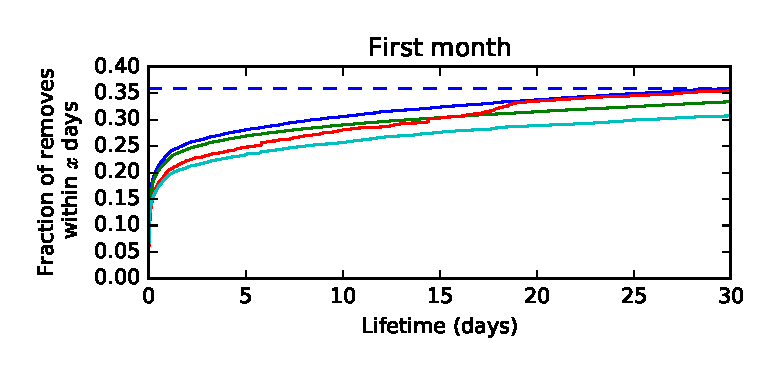
\includegraphics[width=1\textwidth]{assets/irrelevant_identifiers_persistence_cdf_1month_slides}

        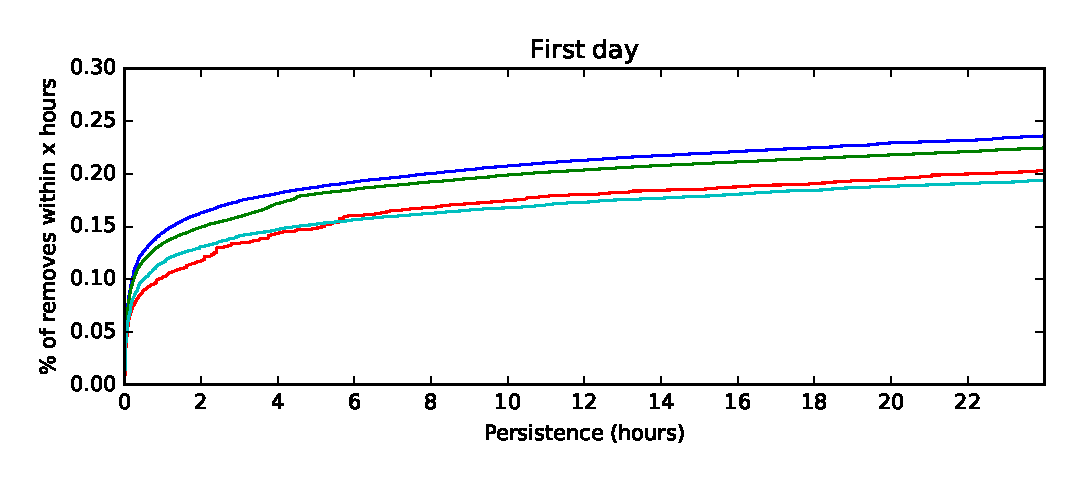
\includegraphics[width=1\textwidth]{assets/irrelevant_identifiers_persistence_cdf_1day_slides}
        \end{figure}
    \end{columns}
\end{frame}

\section{Conclusion}

\begin{frame}[c]
\Huge{\centerline{Conclusion}}
\end{frame}



% \begin{frame}
% \frametitle{The idea}
% \begin{columns}[t] % The "c" option specifies centered vertical alignment while the "t" option is used for top vertical alignment
%
% \column{.5\textwidth} % Left column and width
% \textbf{Past}
% \begin{enumerate}
% \item Relatively small size
% \item (Almost) static network
% \item Nodes have {\color{red}{full}} view of the network
% \end{enumerate}
%
% \column{.5\textwidth} % Right column and width
% \textbf{Now}
% \begin{enumerate}
% \item Big size
% \item Dynamic network
% \item Nodes have {\color{red}{partial}} view of the network
% \end{enumerate}
% \end{columns}\end{frame}
%
%
% \begin{frame}
% \frametitle{Implementation}
% A PSS can be implemented:
% \begin{itemize}
% 	\item as a \textbf{centralized service}: expensive to run reliably
% 	\item using \textbf{gossip protocols}: the most widely adopted solution
% 	\item using \textbf{random walks}: suitable for stable networks
% \end{itemize}
% \end{frame}
%
% \begin{frame}
% \frametitle{The problems}
% \begin{columns}[t] % The "c" option specifies centered vertical alignment while the "t" option is used for top vertical alignment
%
% \column{.5\textwidth} % Left column and width
% \textbf{First problem:}
%
% \begin{itemize}
% 	\item Network Address Translation (NAT)
% 	\item Firewall
% 	\item Antivirus
% 	\item etc etc..
% \end{itemize}
%
% \pause
% \textbf{Solution:}
%
% Gossip-based NAT-aware Peer Sampling Service
%
%
% \column{.5\textwidth} % Right column and width
% \textbf{Second problem:}
% \begin{itemize}
% 	\item Require peers to frequently establish network connections and exchange messages with nodes that support direct connectivity
% 	\item It is a complex and costly procedure!
% \end{itemize}
% \pause
% \textbf{Solution:}
%
% Wormhole Peer Sampling Service!
%
% \end{columns}
% \end{frame}
%
% %-----------------------------------------------------------------------------------------------------------------------------
% \subsection{WPSS}
%
% \begin{frame}
% \begin{itemize}
% 	\item Published in 2013
% 	\item It has the same levels of samples' freshness  of the other PSSes, while the connection establishment rate is decreased by one order of magnitude
% 	\pause
% 	\item \textbf{Main idea}: to divide the service into two layers
% \end{itemize}
% \end{frame}
%
% \begin{frame}
% \frametitle{Overlays}
%
% % \begin{figure}
% % \includegraphics[keepaspectratio=true, width=\textwidth]{images/overlay}
% % \end{figure}
%
% \end{frame}
%
% %-----------------------------------------------------------------------------------------------------------------------------
% \section{WebRTC}
%
% \begin{frame}[c]
% \Huge{\centerline{WebRTC}}
%
% \end{frame}
%
%
% \begin{frame}\frametitle{Three main tasks}
% \begin{itemize}
%   \item Acquiring audio and video: getting access to the microphone or camera, getting a streaming of media for either of them
%   \item Communicating audio and video: being able to connect to another WebRTC end-point through Internet, and send audio and video stream in real-time
%   \item Communicating generic data: not only audio and video, but for any arbitrary application data
% \end{itemize}
% \end{frame}
%
% \begin{frame}\frametitle{Three JavaScript APIs}
%
% \begin{itemize}
%   \item\textbf{\textsf{MediaStream} (aka getUserMedia)}
%   \item\textbf{\textsf{RTCPeerConnection}}
%   \item\textbf{\textsf{RTCDataChannel}}
% \end{itemize}
% \end{frame}
%
% %-----------------------------------------------------------------------------------------------------------------------------
% \subsection{Signaling}
%
% \begin{frame}\frametitle{Signaling}
%
% Abstract Signaling
% \begin{itemize}
%   \item Need to exchange ``session description'' objects:
%   \begin{itemize}
%     \item What formats I support, what I want to send
%     \item Network information for peer-to-peer setup
%   \end{itemize}
%   \item Can use any messaging mechanism
%   \item Can use any messaging protocol
% \end{itemize}
% \end{frame}
%
%
% \begin{frame}[c]\frametitle{Signaling}
%
% % \begin{figure}
% % \centering
% % \includegraphics[width=0.9\textwidth]{images/jsep}
% % \end{figure}
%
% \end{frame}
%
% %-----------------------------------------------------------------------------------------------------------------------------
% \subsection{STUN and TURN Servers}
%
% \begin{frame}[t]\frametitle{STUN and TURN Servers}
% % \begin{figure}
% % \centering
% % \includegraphics[keepaspectratio=true, width=0.9\textwidth]{images/noSTUNorTURN}
% % \end{figure}
% \end{frame}
%
%
%
% % \begin{frame}[t]\frametitle{STUN and TURN Servers}
% % \begin{figure}
% % \centering
% % \includegraphics[keepaspectratio=true, width=0.9\textwidth]{images/firewall}
% % \end{figure}
% % \end{frame}
% %
% % \begin{frame}[t]\frametitle{STUN and TURN Servers}
% % \begin{figure}
% % \centering
% % \includegraphics[keepaspectratio=true, width=0.9\textwidth]{images/turn}
% % \end{figure}
% % \end{frame}
%
%
% %-----------------------------------------------------------------------------------------------------------------------------
% \subsection{EasyRTC}
%
% \begin{frame}\frametitle{Back to reality: EasyRTC Framework}
% \begin{itemize}
%   \item Establishing a connection between two peers in WebRTC is not so simple.
%   \item With power comes complexity
%   \item To hide that complexity, Priologic\footnote{A team of Canadian software developers. More information: \url{https://www.priologic.com}} has built the EasyRTC framework.
%   \item Tracker
% \end{itemize}
% \end{frame}
%
%
% %-----------------------------------------------------------------------------------------------------------------------------
% \section{Evaluation}
%
% \begin{frame}[c]
% \Huge{\centerline{Evaluation}}
%
% \end{frame}
%
% \begin{frame}\frametitle{Environment}
% Emulation environment:
% \begin{itemize}
%   \item $N = 1000$
%   \item $View$ $Size = 50$
%   \item $TTL = 100$
% \end{itemize}
% \end{frame}
%
% %-----------------------------------------------------------------------------------------------------------------------------
% \subsection{Freshness}
%
% \begin{frame}
% \frametitle{Average hop count}
%
% % \begin{figure}
% % \centering
% % \begin{subfigure}{.5\textwidth}
% %   \centering
% %   \includegraphics[keepaspectratio=true, width=1\linewidth]{images/average_hop_count}
% %   \caption{}
% %   \label{fig:my_average_hop_count}
% % \end{subfigure}%
% % \begin{subfigure}{.5\textwidth}
% %   \centering
% %   \includegraphics[keepaspectratio=true, width=1\linewidth]{images/paper_average_hop_count}
% %   \caption{}
% %   \label{fig:paper_average_hop_count}
% % \end{subfigure}
% % \caption{Measure of the average hop count, as well as the $90^{th}$ and $99^{th}$ percentile.~\ref{fig:my_average_hop_count} represents our result,~\ref{fig:paper_average_hop_count} is the test reported in the paper.}
% % \label{fig:freshness}
% % \end{figure}
%
% \end{frame}
%
% %-----------------------------------------------------------------------------------------------------------------------------
% \subsection{Robustness}
%
% \begin{frame}
% \frametitle{Hop count in a flash crowd scenario}
%
% % \begin{figure}
% % \centering
% % \begin{subfigure}{.5\textwidth}
% %   \centering
% %   \includegraphics[keepaspectratio=true, width=1\linewidth]{images/average_hop_count_flash_crowd_1impl}
% %   \caption{}
% %   \label{fig:average_hop_count_flash_crowd_1impl}
% % \end{subfigure}%
% % \begin{subfigure}{.5\textwidth}
% %   \centering
% %   \includegraphics[keepaspectratio=true, width=1\linewidth]{images/paper_average_hop_count_flash_crowd}
% %   \caption{}
% %   \label{fig:paper_average_hop_count_flash_crowd}
% % \end{subfigure}
% % \caption{Average hop count in a flash crowd scenario.~\ref{fig:average_hop_count_flash_crowd_1impl} represents our result,~\ref{fig:paper_average_hop_count_flash_crowd} is the test reported in the paper.}
% % \label{fig:robustness_hop_count_flash_crowd}
% % \end{figure}
%
% \end{frame}
%
% \begin{frame}
% \frametitle{Average in-degree}
%
% % \begin{figure}
% % \centering
% % \begin{subfigure}{.5\textwidth}
% %   \centering
% %   \includegraphics[keepaspectratio=true, width=1\linewidth]{images/average_indegree}
% %   \caption{}
% %   \label{fig:average_indegree}
% % \end{subfigure}%
% % \begin{subfigure}{.5\textwidth}
% %   \centering
% %   \includegraphics[keepaspectratio=true, width=1\linewidth]{images/paper_average_indegree}
% %   \caption{}
% %   \label{fig:paper_average_indegree}
% % \end{subfigure}
% % \caption{Average in-degree in a flash crowd scenario.~\ref{fig:average_indegree} represents our result,~\ref{fig:paper_average_indegree} is the test reported in the paper.}
% % \label{fig:robustness_indegree_flash_crowd}
% % \end{figure}
%
% \end{frame}
%
% \begin{frame}
% \frametitle{Hop count in a massive failure scenario}
%
% % \begin{figure}
% % \centering
% % \begin{subfigure}{.5\textwidth}
% %   \centering
% %   \includegraphics[keepaspectratio=true, width=1\linewidth]{images/average_hop_count_failures_1impl}
% %   \caption{}
% %   \label{fig:average_hop_count_failures_1impl}
% % \end{subfigure}%
% % \begin{subfigure}{.5\textwidth}
% %   \centering
% %   \includegraphics[keepaspectratio=true, width=1\linewidth]{images/paper_average_hop_count_failures}
% %   \caption{}
% %   \label{fig:paper_average_hop_count_failures}
% % \end{subfigure}
% % \caption{Average hop count in a flash crowd scenario.~\ref{fig:average_hop_count_failures_1impl} represents our result,~\ref{fig:paper_average_hop_count_failures} is the test reported in the paper.}
% % \label{fig:robustness_hop_count_failures}
% % \end{figure}
%
% \end{frame}
%
% \begin{frame}
% \frametitle{Average number of dead links}
%
% % \begin{figure}
% % \centering
% % \begin{subfigure}{.5\textwidth}
% %   \centering
% %   \includegraphics[keepaspectratio=true, width=1\linewidth]{images/average_dead_links}
% %   \caption{}
% %   \label{fig:average_dead_links}
% % \end{subfigure}%
% % \begin{subfigure}{.5\textwidth}
% %   \centering
% %   \includegraphics[keepaspectratio=true, width=1\linewidth]{images/paper_average_dead_links}
% %   \caption{}
% %   \label{fig:paper_average_dead_links}
% % \end{subfigure}
% % \caption{Average number of dead links in a flash crowd scenario.~\ref{fig:average_dead_links} represents our result,~\ref{fig:paper_average_dead_links} is the test reported in the paper.}
% % \label{fig:robustness_dead_links_failures}
% % \end{figure}
%
% \end{frame}
%
% %-----------------------------------------------------------------------------------------------------------------------------
% \subsection{Churn}
%
% \begin{frame}
% \frametitle{Hop count with different levels of churn}
%
% % \begin{figure}
% % \centering
% % \begin{subfigure}{.5\textwidth}
% %   \centering
% %   \includegraphics[keepaspectratio=true, width=1\linewidth]{images/average_hop_count_churn_1impl}
% %   \caption{}
% %   \label{fig:average_hop_count_churn_1impl}
% % \end{subfigure}%
% % \begin{subfigure}{.5\textwidth}
% %   \centering
% %   \includegraphics[keepaspectratio=true, width=1\linewidth]{images/paper_average_hop_count_churn}
% %   \caption{}
% %   \label{fig:paper_average_hop_count_churn}
% % \end{subfigure}
% % \caption{Average hop count under varying levels of churn. ~\ref{fig:average_hop_count_churn_1impl} represents our result,~\ref{fig:paper_average_hop_count_churn} is the test reported in the paper.}
% % \label{fig:robustness_hop_count_churn}
% % \end{figure}
%
% \end{frame}
%
% %-----------------------------------------------------------------------------------------------------------------------------
% \section{Gossip-based aggregation protocol}
%
% \begin{frame}[c]
%
% \Huge{\centerline{Gossip-based aggregation protocol}}
%
% \end{frame}
%
%
% \begin{frame}
% \frametitle{The idea}
%
% Aggregation is a common name for a set of functions that provide a summary of some global system property.
%
% \begin{itemize}
%   \item They allow local access to global information in order to simplify the task of controlling, monitoring and optimization in distributed applications
% \end{itemize}
%
% Examples of aggregation functions include network size, total free storage, maximum load, average uptime, etc.
%
% \end{frame}
%
% \begin{frame}
% \frametitle{The idea}
% \begin{itemize}
%   \item The core of the protocol is a simple gossip-based communication scheme
%   \item During this communication the nodes update their local approximate values
%   \item All the approximate values in the system will quickly converge to the desired aggregate value
% \end{itemize}
% \end{frame}
%
% \begin{frame}
% \frametitle{Our case}
% We consider the same network of the tests.
% \begin{itemize}
%   \item Each node in the network holds a numeric value
%   \item We want to calculate the average among the nodes
% \end{itemize}
%
% In a practical setting, this value can characterize any aspect of the node or its environment (e.g., the load at the node, available storage space, temperature measured by a sensor network, etc.).
%
% \end{frame}
%
% \begin{frame}
% \frametitle{First case}
%
% \begin{itemize}
%   \item All the nodes start with a random value between 0 and 1
%   \item The expected output is the average over all these local values.
% \end{itemize}
% \end{frame}
%
%
% \begin{frame}
% \frametitle{First case result}
% \begin{table}
% \begin{tabular}{l l l}
% \toprule
% \textbf{Round} & \textbf{Minimum} & \textbf{Maximum}\\
% \midrule
% 1 & 0.018574914802 & 0.996774217487 \\
% 2 & 0.070221341605 & 0.915147169418 \\
% 3 & 0.230152943376 & 0.833776234641 \\
% 4 & 0.289588175545 & 0.709077004544 \\
% 5 & 0.403064215889 & 0.597074271548 \\
% 6 & 0.450672692662 & 0.554978304631 \\
% ... & ... & ... \\
% 17  & 0.500661439413 & 0.500804356814 \\
% 18  & 0.500675542521 & 0.500750820268 \\
% 19  & 0.500703691477 & 0.5007381087 \\
% 20  & 0.500709860355 & 0.500727408936 \\
% \bottomrule
% \end{tabular}
% \caption{Global average, minimum and maximum in each round.}
% \end{table}
% \end{frame}
%
% \begin{frame}
% \frametitle{First case}
%
% % \begin{figure}[p]
% % \centering
% % \includegraphics[keepaspectratio=true, width=0.8\linewidth]{images/aggregation_average}
% % \caption{Average evolution with error bars.}
% % \label{fig:aggregation_average}
% % \end{figure}
% \end{frame}
%
% \begin{frame}
% \frametitle{First case}
%
% % \begin{figure}[p]
% % \centering
% % \includegraphics[keepaspectratio=true, width=0.8\textwidth]{images/aggregation_standard_deviation}
% % \caption{Standard deviation evolution.}
% % \label{fig:aggregation_standard_deviation}
% % \end{figure}
% %
% \end{frame}
%
% \begin{frame}
% \frametitle{Second case}
%
% \begin{itemize}
%   \item One node starts with 1 and the others with 0.
%   \item The expected output is $1/N$, and if we do the inverse we obtain the total number of nodes present in the network (\textbf{Counting protocol}).
% \end{itemize}
% \end{frame}
%
% \begin{frame}
% \frametitle{Second case result}
% \begin{table}
% \begin{tabular}{l l}
% \toprule
% \textbf{Round} & \textbf{Average}\\
% \midrule
% 1 & 0.0012617200674100 \\
% 2 & 0.0015042163745800 \\
% 3 & 0.0013683466120000 \\
% 4 & 0.0011746396263000 \\
% 5 & 0.0009807697464010 \\
% 6 & 0.0010497184912800 \\
% ... & ... \\
% 17  & 0.0010094031404220 \\
% 18  & 0.0010013031404250 \\
% 19  & 0.0010014001404220 \\
% 20  & 0.0010014031404250 \\
% \bottomrule
% \end{tabular}
% \caption{Global average in each round.}
% \end{table}
% \end{frame}
%
%
% \begin{frame}
% \frametitle{Second case}
% %
% % \begin{figure}[p]
% % \centering
% % \includegraphics[keepaspectratio=true, width=0.8\textwidth]{images/counting_average}
% % \caption{Average evolution with error bars.}
% % \label{fig:counting_average}
% % \end{figure}
%
% \end{frame}
%
%
% \begin{frame}
% \frametitle{Second case}
% %
% % \begin{figure}[p]
% % \centering
% % \includegraphics[keepaspectratio=true, width=0.8\textwidth]{images/counting_standard_deviation}
% % \caption{Standard deviation evolution.}
% % \label{fig:counting_standard_deviation}
% % \end{figure}
%
% \end{frame}
% %-----------------------------------------------------------------------------------------------------------------------------
%
% \begin{frame}
% \Huge{\centerline{The End}}
% \end{frame}
%
% %-----------------------------------------------------------------------------------------------------------------------------
%
% \appendix
%
% \begin{frame}[fragile] % Need to use the fragile option when verbatim is used in the slide
% \frametitle{The algorithm}
%
% \begin{algorithm}[H]
%   \SetKwProg{Upon}{upon}{ do}{end}
%   \SetKwProg{Every}{every}{ do}{end}
%
%   \Upon{wormholeFailure}{
%     $wormhole \leftarrow tracker.getNewWormhole()$\;
%     $connect(wormhole)$\;
%   }
%
%   \Upon{baseOverlayFailure}{
%     $peer \leftarrow tracker.getNewPeer()$\;
%     $connect(peer)$
%   }
%  \caption{Wormhole peer sampling}
% \end{algorithm}
%
% \end{frame}
%
% \begin{frame}[fragile] % Need to use the fragile option when verbatim is used in the slide
% \frametitle{The algorithm}
%
% \begin{algorithm}[H]
%   \SetKwProg{Upon}{upon}{ do}{end}
%   \SetKwProg{Every}{every}{ do}{end}
%
%   \Every{$\Delta_{wh}$ = wormholeTimeout}{
%     $disconnect(wormhole)$\;
%     $wormhole \leftarrow tracker.getNewWormhole()$\;
%     $connect(wormhole)$\;
%   }
%
%   \Every{$\Delta$ = adTimeout}{
%     $ad \leftarrow createAd()$\;
%     $ad.hops \leftarrow 1$\;
%     $sendAdToWormhole(wormhole, ad)$\;
%   }
%   \caption{Wormhole peer sampling}
% \end{algorithm}
%
% \end{frame}
%
% \begin{frame}
% \frametitle{The algorithm}
%
% \begin{algorithm}[H]
%   \SetKwProg{Upon}{upon}{ do}{end}
%   \SetKwProg{Every}{every}{ do}{end}
%
%   \Upon{receivedAd(ad)}{
%     \If{ad.hop = getTTL() $\mid\mid$ acceptAd(ad)}{
%       view.addAd(ad)
%     }\Else{
%       $neighbour \leftarrow getMetropolisHastingsNeighbour()$\;
%       $ad.hop \leftarrow ad.hop + 1$\;
%       $sendAd(neighbour, ad)$\;
%     }
%   }
%   \caption{Wormhole peer sampling}
% \end{algorithm}
% \end{frame}

\begin{frame}[allowframebreaks]{References}
    \bibliographystyle{unsrt}
    \bibliography{biblio}
\end{frame}


\end{document}
